\chapter{Matematický model}
\label{kap:matematicky_model}
Upravme rovnice pre obálku sféry tak, aby zodpovedali obálke elipsoidov. Vezmime elipsoid so škálovaním v smere súradnicových osí konštantnými reálnymi číslami $a,b,c.$ Upravme škálovanie elipsoidu tak, aby $a$, škálovanie v smere osi $x$ zodpovedalo škálovaniu v dotykovom smere priestorovej krivky $m(t).$
Teda pre elipsoid s rovnicou
\begin{equation*}
\frac{{(x - m_1(t))^2}}{{a^2}} + \frac{{(y - m_2(t))^2}}{{b^2}} + \frac{{(z - m_3(t))^2}}{{c^2}}= 1
\end{equation*} 
zmeníme štandardnú bázu $\vec{e}_1, \vec{e}_2, \vec{e}_3$ na bázu Frenetovho repéra $\vec{t}, \vec{n}, \vec{b}$ v každom bode krivky $m(t).$ Naše očakávanie je, že obálku  elipsoidu škálovaného v dotykovom smere budeme môcť zostrojiť znova ako obálku kružníc, a teda, deriváciou jednoparametrického systému elipsoidov je podľa parametra $t$ bude opäť rovina. V ďalších výpočtoch budeme parameter $t$ pre väčšiu prehľadnosť zápisov vynechávať.
\section{Obálka sfér}
Obálku sfér vieme zapísať skalárnym súčinom, no existuje však aj všeobecný zápis pre plochy druhého rádu, a to maticový 
$$
S: X^TM(t)X = 0,
$$
kde $ X = (x, y, z)^T \in \mathbb{R}^3 $ a $M(t) $ je symetrická matica rozmeru $4x4, $ ktorej koeficienty sú závislé od $t \in I$.
Rovnicu jednoparametrického systému sfér $S$
$$ x^2 +y^2 +z^2 -2xm_1 -2ym_2 - 2zm_3 + m_1^2 + m_2^2 + m_3^2 - r^2 =0
,$$
tak vieme zapísať ako
$$
\left(\begin{matrix} x \\ y \\ z  \\ 1
\end{matrix} \right)^T \left(\begin{matrix} 
1 & 0 & 0 & - m_1 \\
0 & 1 & 0 & - m_2 \\
0 & 0 & 1 & - m_3 \\
- m_1 & - m_2 & - m_3 &  m_1^2 + m_2^2 + m_3^2 - r^2 \\
\end{matrix} \right)\left(\begin{matrix} x \\ y \\ z \\ 1
\end{matrix} \right) = 0. 
$$
Deriváciu jednoparametrického systému sfér $\dot{S}$
$$
-2x\dot{m}_1 -2y\dot{m}_2 - 2z\dot{m}_3 + 2m_1\dot{m_1} + 2m_2\dot{m_2} + 2m_3\dot{m_3} - 2r\dot{r} = 0
$$
možno tiež zapísať v tvare  $X^T\dot{M}(t)X = 0,$
kde $\dot{M}(t)= \dfrac{\partial M(t)}{\partial t}.$
$$
\left(\begin{matrix} x \\ y \\ z  \\ 1
\end{matrix} \right)^T \left(\begin{matrix} 
0 & 0 & 0 & - \dot{m}_1 \\
0 & 0 & 0 & - \dot{m}_2 \\
0 & 0 & 0 & - \dot{m}_3 \\
- \dot{m}_1 & - \dot{m}_2 & - \dot{m}_3 &  2m_1\dot{m_1} + 2m_2\dot{m_2} + 2m_3\dot{m_3} - 2r\dot{r} \\
\end{matrix} \right)\left(\begin{matrix} x \\ y \\ z \\ 1
\end{matrix} \right) = 0,
$$
Matica $\dot{M}(t)$ reprezentuje v každom $t \in I $ rovinu, ktorej normálový vektor $\vec{N} $ je $(-2\dot{m}_1, -2\dot{m}_2, -2\dot{m}_3).$ Vektor $\vec{N}$ je lineárne závislý s dotykovým vektorom $\dot{m}$ ku krivke $m.$
\section{Obálka elipsoidov}
Rovnako zapíšme rovnicu jednoparametrického systému elipsoidov $Q$
$$ \frac{x^2}{a^2} + \frac{y^2}{b^2} + \frac{z^2}{c^2} - 2 \frac{xm_1}{a^2} - 2 \frac{ym_2}{b^2} - 2 \frac{zm_3}{c^2} + \frac{m_1^2}{a^2} + \frac{m_2^2}{b^2} + \frac{m_3^2}{c^2} - 1 = 0,$$
$$
\left(\begin{matrix} x \\ y \\ z  \\ 1
\end{matrix} \right)^T \left(\begin{matrix} 
\frac{1}{a^2} & 0 & 0 & \frac{-m_1}{a^2} \\
0 & \frac{1}{b^2} & 0 & \frac{-m_2}{b^2} \\
0 & 0 & \frac{1}{c^2} & \frac{-m_3}{c^2} \\
\frac{-m_1}{a^2} & \frac{-m_2}{b^2} & \frac{-m_3}{c^2} & \frac{m_1}{a^2} + \frac{m_2}{b^2} + \frac{m_3}{c^2} - 1 \\
\end{matrix} \right)\left(\begin{matrix} x \\ y \\ z \\ 1
\end{matrix} \right) = 0,
$$
potom derivácia jednoparametrického systému elipsoidov, ktorú označíme $\dot{Q} = \dfrac{\partial Q(t)}{\partial t}$
$$
-\frac{\dot{m}_1x}{a^2} + \frac{\dot{m}_2y}{b^2} + \frac{\dot{m}_3z}{c^2} + \frac{m_1\dot{m}_1}{a^2} + \frac{m_2 \dot{m}_2}{b^2} + \frac{m_3 \dot{m}_3}{c^2} = 0,
$$
má v maticovom zápise tvar
$$
\left(\begin{matrix} x \\ y \\ z  \\ 1
\end{matrix} \right)^T \left(\begin{matrix} 
0 & 0 & 0 & \frac{-\dot{m}_1}{a^2} \\
0 & 0 & 0 & \frac{-\dot{m}_2}{b^2} \\
0 & 0 & 0 & \frac{-\dot{m}_3}{c^2} \\
\frac{-\dot{m}_1}{a^2} & \frac{-\dot{m}_2}{b^2} & \frac{-\dot{m}_3}{c^2} & \frac{2m_1\dot{m}_1}{a^2} + \frac{2m_2 \dot{m}_2}{b^2} + \frac{2m_3 \dot{m}_3}{c^2}\\
\end{matrix} \right)\left(\begin{matrix} x \\ y \\ z \\ 1
\end{matrix} \right) = 0.
$$
$ \dot{Q}$ je rovina kolmá na dotykový vektor $\dot{m}(t), $ práve vtedy keď vektory $(\dot{m}_1, \dot{m}_2, \dot{m}_3) $ a $(\frac{\dot{m}_1}{a^2}, \frac{\dot{m}_2}{b^2}, \frac{\dot{m}_3}{c^2}) $ sú lineárne závislé. Ak budeme elipsoid škálovať tak, že $a, b, c$ budú škálovacie faktory také, aby sa elipsoid naškáloval v dotykovom smere, tak kolmá rovina na dotykový vektor vytne kružnicu, pretože elipsoid je v ostatných smeroch homogénny. Vyriešme toto odvodenie pre jednoduchší prípad, a to prípad elíps.

\section{Obálka elíps}
\subsection{Zmena bázy}
Nech $m(t) \colon  I \subseteq \mathbb{R} \rightarrow \mathbb{R}^2$ je aspoň dvakrát diferencovateľná krivka, položme elipsu $Q$ s osami $a_0, b_0 \in \mathbb{R}$ na túto krivku v každom bode $t \in I.$
\begin{equation*}
\frac{{(x - m_1(t))^2}}{a_0^2} + \frac{{(y - m_2(t))^2}}{b_0^2} = 1
\end{equation*}
Matica prechodu k novej báze je tvaru
$$
A(t) = \left(\begin{matrix} \vec{t}(t) \quad \vec{n}(t)
\end{matrix} \right),
$$
čo po rozpísaní do súradníc $\vec{t}(t) = \frac{1}{ \| \dot{m}(t) \|}( \dot{m}_1(t),  \dot{m}_2(t))$ a $\vec{n}(t) = \frac{1}{ \| \dot{m}(t) \|}( -\dot{m}_2(t),  \dot{m}_1(t))$ dáva 
$$
A(t) = \frac{1}{ \| \dot{m}(t) \|} \left(\begin{matrix}
   \dot{m}_1(t) & n_1(t) \\
   \dot{m}_2(t) & n_2(t)
\end{matrix} \right).
$$
Keďže sme maticu $A(t)$ zostrojili tak, aby bola ortogonálna, ľahko dostávame aj vyjadrenie inverznej matice
$$
A^{-1}(t) = A^{T}(t) = \frac{1}{ \| \dot{m}(t) \|} \left(\begin{matrix}
  \dot{m}_1(t) & \dot{m}_2(t) \\
    n_1(t) & n_2(t)
\end{matrix}\right).
$$
Vyjadrime elipsu $Q$ v novej báze $ u, v$ nasledovnou transformáciou
\begin{align*}
\frac{u^2(t)}{a^2} + \frac{v^2(t)}{b^2} = 1,
\end{align*}
kde 
$$
\left(\begin{matrix}
u(t) \\
v(t)
\end{matrix}\right) = \frac{1}{ \| \dot{m}(t) \|}
\left(\begin{matrix}
  \dot{m}_1(t) & \dot{m}_2(t) \\
    n_1(t) & n_2(t)
\end{matrix}\right)
\left(\begin{matrix}
x-m_1(t) \\
y-m_2(t) \\
\end{matrix}\right).
$$
Elipsa $Q$ sa potom transformuje na 
\begin{align} 
\label{eq:elipsa_v_novej_baze}
&\frac{1}{\|{m}\|^2} \left( (x - m_1)^2 \left( \frac{{\dot{m}_1}^2}{a^2} + \frac{{\dot{m}_2}^2}{b^2} \right) + (y - m_2)^2 \left( \frac{{\dot{m}_2}^2}{a^2} + \frac{{\dot{m}_1}^2}{b^2} \right) \right) \\
+ &\frac{1}{\|{m}\|^2} \left( 2(x - m_1)(y - m_2)\dot{m}_1\dot{m}_2 \left( \frac{1}{a^2} - \frac{1}{b^2} \right) \right) - 1 = 0,
\end{align}
po miernej úprave tak dostávame výraz
\begin{align*} 
&\frac{1}{a^2b^2\|m\|^2} \left( (x - m_1)^2 \left( b^2 \dot{m}_1^2 + a^2 \dot{m}_2^2 \right) + (y - m_2)^2 \left( a^2 \dot{m}_1^2 + b^2 \dot{m}_2^2 \right) \right) \\
+ &\frac{1}{a^2b^2\|\dot{m}\|^2} \left( 2(b^2 - a^2)(x - m_1)(y - m_2)\dot{m}_1\dot{m}_2 \right) - 1 = 0,
\end{align*}
kde konštanta $a$ zabezpečí škálovanie elipsy v dotykovom smere a konštanta $b$ určí škálovanie v normálovom smere. Výber orientácie normály nemá na výsledok žiaden vplyv. Štandardne uvažujeme $\vec{n}=(-\dot{m}_2, \dot{m}_1).$

\begin{example}[Parabola]
Majme parabolu s parametrizáciou $m(t)=(t, t^2), $ kde $\dot{m}(t)=(1, 2t).$ Transformujme elipsu v stredovom zápise so škálovaním v smere súradnicových osí
\begin{equation*}
\frac{(x - t)^2}{a_0^2} + \frac{(y - t^2)^2}{b_0^2} = 1
\end{equation*}
na elipsu so škálovaním $a$ v dotykovom a $b$ v normálovom smere
\begin{align*}
&\frac{1}{a^{2} b^{2}\left(4 t^{2} + 1\right)} \left( (x-t)^2 (b^2 + a^{2} 4t^2) + (y-t^2)^2 (a^2 + b^2 4t^2) \right)\\
+ &\frac{1}{a^{2} b^{2}\left(4 t^{2} + 1\right)} \left( 2(b^2 - a^2)(x-t)(y-t^2)2t \right) - 1 = 0.
\end{align*}
\end{example}

\subsection{Výpočet obálky elíps}
Prepíšme rovnicu \ref{eq:elipsa_v_novej_baze} do maticového zápisu. Máme kužeľosečku $Q$ tvaru $$
Ax^2 + Bxy + Cy^2 + Dx + Ey + F = 0,$$
ktorá má v maticovom tvare vyjadrenie 
$$
\left(\begin{matrix} x \\ y \\ 1 
\end{matrix} \right)^T \left(\begin{matrix} 
A & \frac{B}{2} & \frac{D}{2} \\
\frac{B}{2} & C & \frac{E}{2} \\
\frac{D}{2} & \frac{E}{2} & F 
\end{matrix} \right)\left(\begin{matrix} x \\ y \\ 1 
\end{matrix} \right) = 0,
$$
Všetky koeficienty matice $M(t)$ sú závislé od $t$ a majú nasledovný tvar
\begin{align*}
A &= \frac{b^2 \dot{m}_1^2 + a^2 \dot{m}_2^2}{a^2b^2 \| m \|^2} \\
B &= \frac{2(b^2-a^2)\dot{m}_1 \dot{m}_2}{a^2b^2 \| m \|^2} \\
C &= \frac{a^2 \dot{m}_1^2 + b^2 \dot{m}_2^2}{a^2b^2\| m\|^2} \\
D &= \frac{- 2m_1 \left( b^2 \dot{m}_1^2 + a^2 \dot{m}_2^2 \right) - 2 \left(b^2 - a^2 \right) m_2 \dot{m}_1 \dot{m}_2 }{a^2b^2\| m \|^2} \\
E &= \frac{- 2m_2 \left( a^2 \dot{m}_1^2 + b^2 \dot{m}_2^2 \right) - 2 \left(b^2 - a^2 \right) m_1 \dot{m}_1 \dot{m}_2 }{a^2b^2\| m \|^2} \\
F &= \frac{\dot{m}_1^2 (b^2 m_1^2 + a^2 m_2^2 - a^2b^2) + 2 (b^2 - a^2) m_1 m_2 \dot{m}_1 \dot{m}_2 + \dot{m}_2^2 (a^2 m_1^2 + b^2 m_2^2 - a^2b^2) }{a^2b^2\| \dot{m}  \|^2}  -  1  \\
\end{align*}
Pozrime sa deriváciu jednoparametrického systému elíps podľa parametra $t.$ Máme teda kužeľosečku $\dot{Q}$ tvaru 
$$
\dot{A}x^2 + \dot{B}xy + \dot{C}y^2 + \dot{D}x + \dot{E}y + \dot{F} = 0$$
kde $\dot{A}, \dots, \dot{F}$ sú koeficienty matice $\dot{M}(t).$

\begin{align*}
\dot{A} &= \frac{2 (a^{2} \dot{m}_{1} \ddot{m}_{2} - a^{2} \ddot{m}_{1} \dot{m}_{2} - b^{2} \dot{m}_{1} \ddot{m}_{2} + b^{2} \ddot{m}_{1} \dot{m}_{2}) \dot{m}_{1} \dot{m}_{2}}{a^2b^2 \| m \|^4} \\
\dot{B} &= 2\frac{(2 a^{2} (\dot{m}_{1} \ddot{m}_{1} + \dot{m}_{2} \ddot{m}_{2}) \dot{m}_{1} \dot{m}_{2} - a^{2} (\dot{m}_{1} \ddot{m}_{2} + \ddot{m}_{1} \dot{m}_{2}) (\dot{m}_{1}^{2} + \dot{m}_{2}^{2}) - 2b^{2} (\dot{m}_{1} \ddot{m}_{1} + \dot{m}_{2} \ddot{m}_{2}) \dot{m}_{1} \dot{m}_{2} + b^{2} (\dot{m}_{1} \ddot{m}_{2} + \ddot{m}_{1} \dot{m}_{2}) (\dot{m}_{1})^{2} + \dot{m}_{2}^{2}))}{a^2b^2 \| m \|^4} \\
\dot{C} &= \frac{2 (- a^{2} \dot{m}_{1} \ddot{m}_{2} + a^{2} \ddot{m}_{1} \dot{m}_{2} + b^{2} \dot{m}_{1} \ddot{m}_{2} - b^{2} \ddot{m}_{1} \dot{m}_{2}) \dot{m}_{1} \dot{m}_{2}}{a^2b^2 \| m \|^4} \\
\dot{D} &= \frac{2 \cdot (2 a^{2} (m_{1} \dot{m}_{2} - m_{2} \dot{m}_{1}) (\dot{m}_{1} \ddot{m}_{1} + \dot{m}_{2} \ddot{m}_{2}) \dot{m}_{2} + a^{2} (\| m \|^2 (- 2 m_{1} \dot{m}_{2} \ddot{m}_{2} + m_{2} \dot{m}_{1} \ddot{m}_{2} + m_{2} \ddot{m}_{1} \dot{m}_{2}) + 2 b^{2} (m_{1} \dot{m}_{1} + m_{2} \dot{m}_{2}) (\dot{m}_{1} \ddot{m}_{1} + \dot{m}_{2} \ddot{m}_{2}) \dot{m}_{1} - b^{2} ((\dot{m}_{1})^{2} + (\dot{m}_{2})^{2}) (2 m_{1} \dot{m}_{1} \ddot{m}_{1} + m_{2} \dot{m}_{1} \ddot{m}_{2} + m_{2} \ddot{m}_{1} \dot{m}_{2} + (\dot{m}_{1})^{3} + \dot{m}_{1} (\dot{m}_{2})^{2}))}{a^2b^2 \| m \|^4} \\
\dot{E} &= \frac{2 \cdot (2 a^{2} (- m_{1} \dot{m}_{2} + m_{2} \dot{m}_{1}) (\dot{m}_{1} \ddot{m}_{1} + \dot{m}_{2} \ddot{m}_{2}) \dot{m}_{1} + a^{2} (\| m \|^2 (m_{1} \dot{m}_{1} \ddot{m}_{2} + m_{1} \ddot{m}_{1} \dot{m}_{2} - 2 m_{2} \dot{m}_{1} \ddot{m}_{1}) + 2 b^{2} (m_{1} \dot{m}_{1} + m_{2} \dot{m}_{2}) (\dot{m}_{1} \ddot{m}_{1} + \dot{m}_{2} \ddot{m}_{2}) \dot{m}_{2} - b^{2} ((\dot{m}_{1})^{2} + (\dot{m}_{2})^{2}) (m_{1} \dot{m}_{1} \ddot{m}_{2} + m_{1} \ddot{m}_{1} \dot{m}_{2} + 2 m_{2} \dot{m}_{2} \ddot{m}_{2} + (\dot{m}_{1})^{2} \dot{m}_{2} + (\dot{m}_{2})^{3}))}{a^2b^2 \| m \|^4} \\
\dot{F} &= \frac{2 (a^{2} (\dot{m}_{1} \ddot{m}_{1} + \dot{m}_{2} \ddot{m}_{2}) (- m_{1}^{2} (\dot{m}_{2})^{2} + 2 m_{1} m_{2} \dot{m}_{1} \dot{m}_{2} - m_{2}^{2} (\dot{m}_{1})^{2}) + a^{2} \| m \|^4 (m_{1}^{2} \dot{m}_{2} \ddot{m}_{2} - m_{1} m_{2} \dot{m}_{1} \ddot{m}_{2} - m_{1} m_{2} \ddot{m}_{1} \dot{m}_{2} + m_{2}^{2} \dot{m}_{1} \ddot{m}_{1}) - b^{2} (\dot{m}_{1} \ddot{m}_{1} + \dot{m}_{2} \ddot{m}_{2}) (m_{1}^{2} (\dot{m}_{1})^{2} + 2 m_{1} m_{2} \dot{m}_{1} \dot{m}_{2} + m_{2}^{2} (\dot{m}_{2})^{2}) + b^{2} ((\dot{m}_{1})^{2} + (\dot{m}_{2})^{2}) (m_{1}^{2} \dot{m}_{1} \ddot{m}_{1} + m_{1} m_{2} \dot{m}_{1} \ddot{m}_{2} + m_{1} m_{2} \ddot{m}_{1} \dot{m}_{2} + m_{1} (\dot{m}_{1})^{3} + m_{1} \dot{m}_{1} (\dot{m}_{2})^{2} + m_{2}^{2} \dot{m}_{2} \ddot{m}_{2} + m_{2} (\dot{m}_{1})^{2} \dot{m}_{2} + m_{2} (\dot{m}_{2})^{3}))}{a^2b^2 \| m \|^4}  
\end{align*}
Determinant matice $\dot{M}(t) = 0, $ pre všetky $t$, čo znamená, že kužeľosečka je singulárna.
Pozrime sa na subdeterminant
$$
\dot{M}_{33}(t) = \dot{A} \dot{C} - \frac{\dot{B}^2}{4} =  -\frac{(b^2 - a^2)^2}{a^4b^4} \frac{ (\dot{m_1}\ddot{m_2} - \ddot{m_1}\dot{m_2})^2 + \dot{m_1}\dot{m_2}\ddot{m_1}\ddot{m_2}}{\|m\|^4}.
$$ 
Hodnota $\dot{M}_33(t) < 0, $ pre všetky $t,$ teda kužeľosečka degeneruje na dve rôznobežné priamky.

\section{Obálka elipsoidov}

Na všetky výpočty v tejto kapitole bol použitý voľne dostupný softvér počítačovej algebry Maxima s grafickým užívateľským rozhraním wmMaxima. Celý balík a dokumentácia sú dostupné na \cite{MaximaDoc}, \cite{MaximaDownload}. Rovnice z Maximy boli prevedené do \LaTeX u pomocou Python skriptu \verb|conversion-to-latex.ipynb|, ktorý sa nachádza v GitHub repozitári \url{https://github.com/tutka13/Masters-Thesis/tree/main/symbolic-computations}.

\begin{figure}[h!]
	\centering
	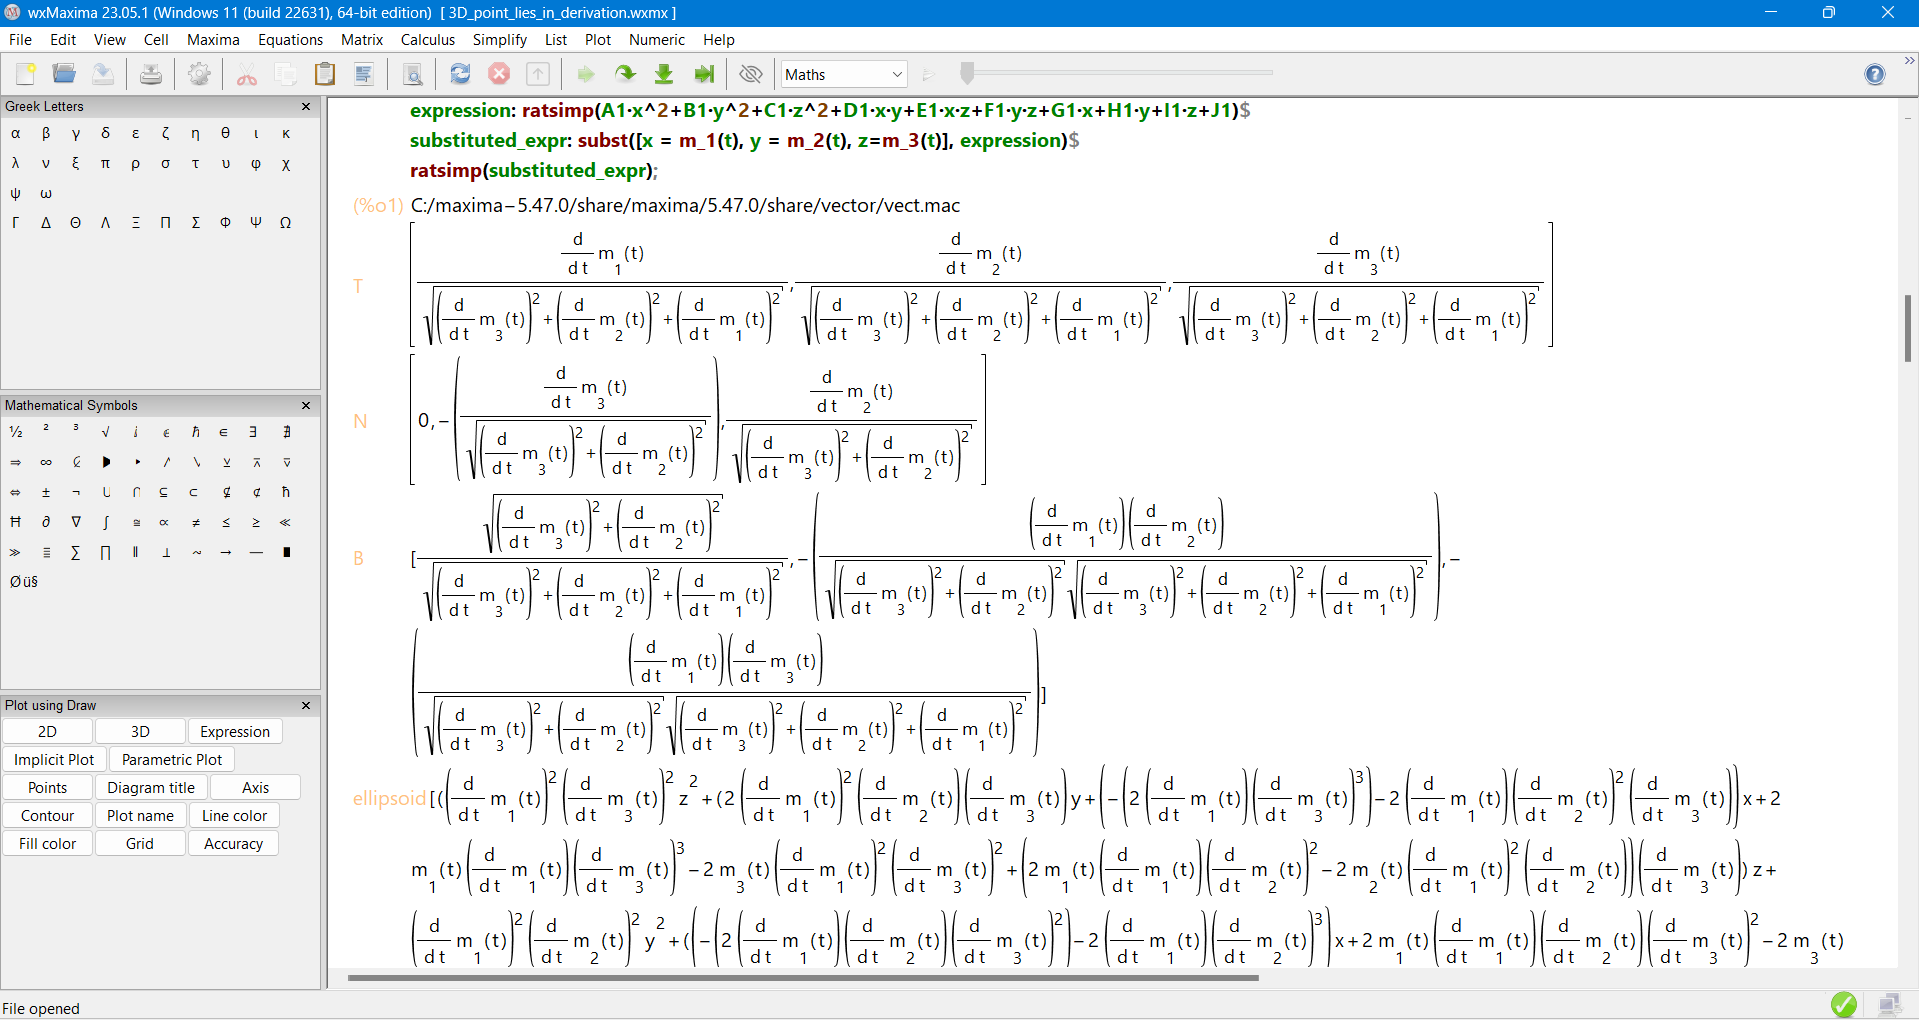
\includegraphics[width=\textwidth]{images/maxima.png}
	\caption[Softvér Maxima.]{Výpočet: bod v paramteri $t$ na krivke $m(t)$ leží v derivácii jednoparametrického systému elipsoidov.}
	\label{fig:3D_point_lies}
\end{figure}

